\documentclass{article}

\usepackage{amsmath,amsfonts,amssymb,amsthm}
\usepackage{enumerate}
\usepackage{arydshln}
\usepackage{listings,color}
\usepackage{graphicx}

\definecolor{dkgreen}{rgb}{0,0.6,0}
\definecolor{gray}{rgb}{0.5,0.5,0.5}
\definecolor{mauve}{rgb}{0.58,0,0.82}

% Opening
\title{Numerical Analysis HW11\\
Ch23 - 2a,7 (pg613)\\
Ch24 - 1,4 (pg635)\\}
\author{Neal D. Nesbitt}

\begin{document}
\maketitle

\theoremstyle{definition}
\newtheorem{problem}{Problem}[section]
\newtheorem{solution}{Solution}[problem]
\renewcommand*{\thesolution}{\theproblem.\alph{solution}}

\lstset{basicstyle=\ttfamily,
		language=Matlab,
		keywordstyle=\color{blue},
		commentstyle=\color{dkgreen},
		stringstyle=\color{mauve},
		identifierstyle=\bf
		}

\setcounter{section}{22}
\section{}

\setcounter{problem}{2}
\begin{problem}
The following ODEs have been proposed as a model of an epidemic:
\begin{align*}
\frac{dS}{dt} &= -aSI		\\
\frac{dI}{dt} &= aSI -rI	\\
\frac{dR}{dt} &= rI
\end{align*}
where $S$ is the number of susceptible individuals, $I$ is the number of infected, $R$ is the number of the recovered, $a$ is the infection rate, and $r$ is the recovery rate. A city has 10,000 people, all of whom are susceptible.
\begin{enumerate}[(a)]
\item If a single infectious individual enters the city at $t=0$, compute the progression of the epidemic until the number of infected individuals falls below 10. Use the following parameters: $a = 0.0002 /(\text{person}\cdot \text{week})$ and $r=0.15/\text{d}$. Develop time series plots of all the state variables. Also generate a phase-plane plot of $S$ versus $I$ versus $R$\\
\item Suppose that after recovery, there is a loss of immunity that causes recovered individuals to become susceptible. This reinfection mechanism can be computed as $\rho R$, where $\rho$ is the reinfection rate. Modify the model to include this mechanism and repeat the computations in (a) using $\rho=0.03/\text{d}$. 
\end{enumerate}
\end{problem}

Let y(1) = S, y(2) = I, y(3) = R, and count $t$ in days. Below are the results for the full and partial immunity models respectively. 

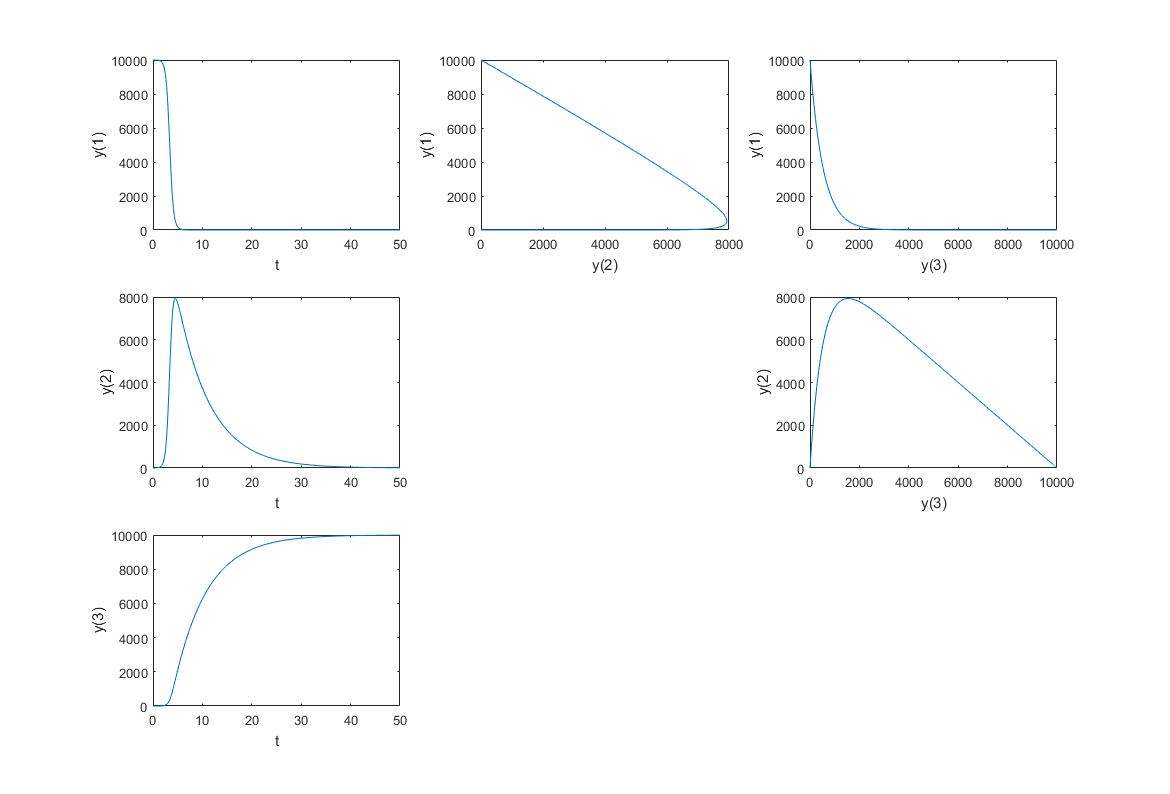
\includegraphics[width=\linewidth]{HW11-epidemic.jpg}

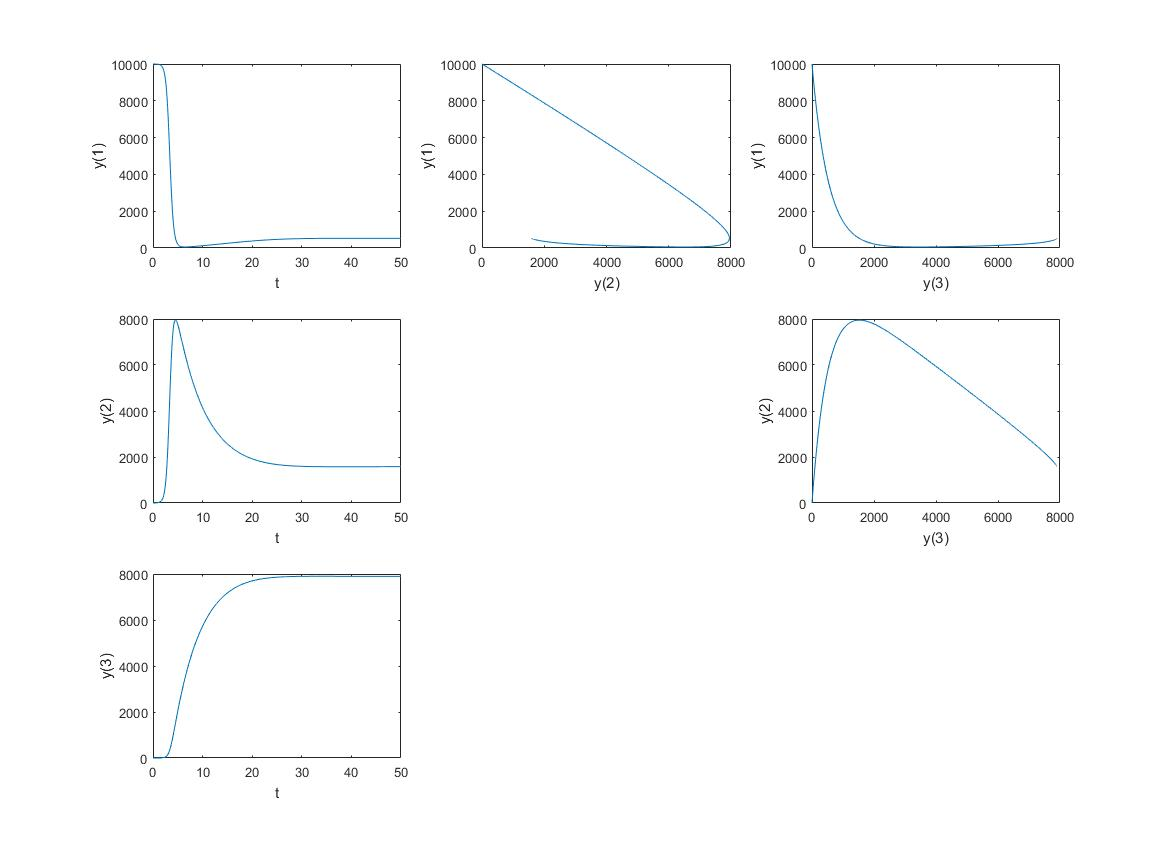
\includegraphics[width=\linewidth]{HW11-epidemic2.jpg}

\setcounter{problem}{6}
\begin{problem}
Given
\begin{align*}
\frac{dx_{1}}{dt} = 999x_{1} + 1999x_{2}\\
\frac{dx_{2}}{dt} = -1000x_{1} -2000x_{2}
\end{align*}
If $x_{1}(0)=x_{2}(0)=1$, obtain a solution from $t=0$ to 0.2 using a step size of 0.05 with
\begin{enumerate}[(a)]
\item the explicit Euler method
\item and the implicit Euler method
\end{enumerate}
\end{problem}

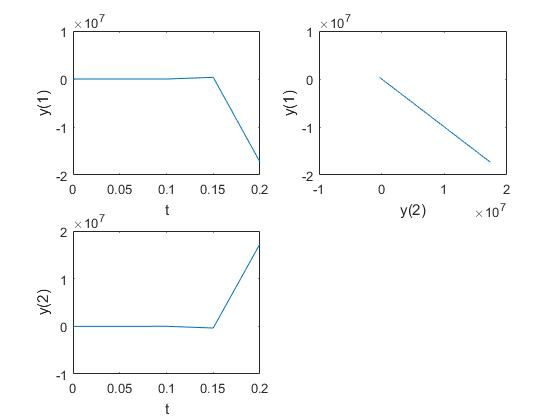
\includegraphics[width=\linewidth]{HW11-ODEsysEx.jpg}
Above is the Explicit version where $y=x$ is the independent variable we solved for.

%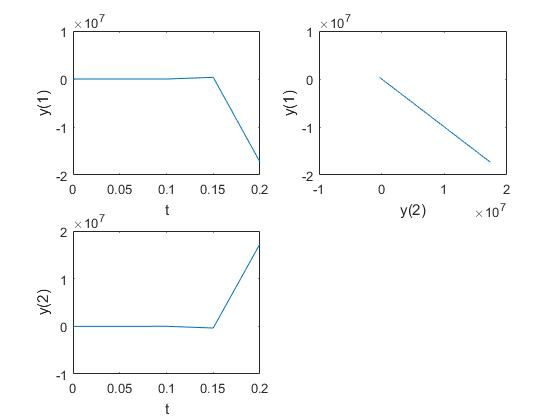
\includegraphics[width=\linewidth]{HW11-ODEsysEx.jpg}
%This is the implicit version with the same labels.

\section{}

\begin{problem}
A steady-state heat balance for a rod can be represented as
\[ \frac{d^{2}T}{dx^{2}} -0.15T = 0 \]
Obtain a solution for a 10-m rod with $T(0)=240$ and $T(10)=150$
\begin{enumerate}[(a)]
\item analytically
\item with the shooting method
\item using the finite difference method with $\Delta x = 1$
\end{enumerate}
\end{problem}

\begin{solution}
\begin{align*}
T(x) &= Ae^{x\sqrt{0.15}} + Be^{-x\sqrt{0.15}}\\
T(0) &= A+B = 240\\
B &= 240-A\\
T(10) &= Ae^{\sqrt{15}} + Be^{-\sqrt{15}} = 150\\
150 &= Ae^{\sqrt{15}} + (240-A)e^{-\sqrt{15}}\\
150 &= 240e^{-\sqrt{15}} +Ae^{\sqrt{15}} -Ae^{-\sqrt{15}}\\
150 &= 240e^{-\sqrt{15}} +2Ai\sin(\sqrt{15})\\
A &= \frac{150 -240e^{-\sqrt{15}}}{2i\sin(\sqrt{15})}\\
A &\approx -1073.43 i\\
B &\approx -1313.43 i
\end{align*}

\[ T(x) = \frac{1073.43 e^{x\sqrt{0.15}} + 1313.43e^{-x\sqrt{0.15}}}{i} \]
\end{solution}

\begin{solution}
content...
\end{solution}

\begin{solution}
Using the finite difference approximation of the second derivative we find
\begin{align*}
\frac{d^{2}T}{dx^{2}} \approx \frac{T_{i-1} -2T_{i} +T_{i+1}}{\Delta x^{2}} &= 0.15T_{i}\\
T_{i-1} -2T_{i} +T_{i+1} &= 0.15T_{i}\Delta x^{2}\\
T_{i-1} -T_{i}(2+0.15\Delta x^{2}) +T_{i+1} &= 0
\end{align*}
So extending this to each step we turn this into a tridiagonal system:
\begin{align*}
\begin{bmatrix}
T_{0}	&	-(2+0.15\Delta x^{2})T_{1}	&	T_{2}	&	0	&\cdots		&	0\\
0		&	T_{1}	&	-(2+0.15\Delta x^{2})T_{2}	&	T_{3}	&\cdots	&	0\\
0	&	\cdots	&	\cdots	&	\cdots	&	\cdots	&	0	\\
0	&	\cdots	&	T_{n-3}	&	-(2+0.15\Delta x^{2})T_{n-2}	&	T_{n-1}	&	0\\
0	&	\cdots	&	0	&	T_{n-2}	&	-(2+0.15\Delta x^{2})T_{n-1}	&	T_{n}
\end{bmatrix}
&=
\begin{bmatrix}
0\\
0\\
\cdots\\
0\\
0\\
\end{bmatrix}
\\
\begin{bmatrix}
-(2+0.15\Delta x^{2})T_{1}	&	T_{2}	&	0	&\cdots	\\
T_{1}	&	-(2+0.15\Delta x^{2})T_{2}	&	T_{3}	&\cdots	\\
\cdots	&	\cdots	&	\cdots	&	\cdots	\\
\cdots	&	T_{n-3}	&	-(2+0.15\Delta x^{2})T_{n-2}	&	T_{n-1}\\
\cdots	&	0	&	T_{n-2}	&	-(2+0.15\Delta x^{2})T_{n-1}
\end{bmatrix}
&=
\begin{bmatrix}
-T_{0}\\
0\\
\cdots\\
0\\
-T_{n}\\
\end{bmatrix}
\\
\begin{bmatrix}
-(2+0.15\Delta x^{2})	&	1	&	0	&\cdots	\\
1	&	-(2+0.15\Delta x^{2})	&	1	&\cdots	\\
\cdots	&	\cdots	&	\cdots	&	\cdots	\\
\cdots	&	1	&	-(2+0.15\Delta x^{2})	&	1\\
\cdots	&	0	&	1	&	-(2+0.15\Delta x^{2})
\end{bmatrix}
\begin{bmatrix}
T_{1}\\
T_{2}\\
\cdots\\
T_{n-2}\\
T_{n-1}
\end{bmatrix}
&=
\begin{bmatrix}
-T_{0}\\
0\\
\cdots\\
0\\
-T_{n}\\
\end{bmatrix}
\end{align*}

Then with the given boundary conditions
\begin{align*}
\begin{bmatrix}
-(2+0.15(10/n)^{2})	&	1	&	0	&\cdots	\\
1	&	-(2+0.15(10/n)^{2})	&	1	&\cdots	\\
\cdots	&	\cdots	&	\cdots	&	\cdots	\\
\cdots	&	1	&	-(2+0.15(10/n)^{2})	&	1\\
\cdots	&	0	&	1	&	-(2+0.15(10/n)^{2})
\end{bmatrix}
\begin{bmatrix}
T_{1}\\
T_{2}\\
\cdots\\
T_{n-2}\\
T_{n-1}
\end{bmatrix}
&=
\begin{bmatrix}
-240\\
0\\
\cdots\\
0\\
-150\\
\end{bmatrix}
\\
\begin{bmatrix}
-(2+15/n^{2})	&	1	&	0	&\cdots	\\
1	&	-(2+15/n^{2})	&	1	&\cdots	\\
\cdots	&	\cdots	&	\cdots	&	\cdots	\\
\cdots	&	1	&	-(2+15/n^{2})	&	1\\
\cdots	&	0	&	1	&	-(2+15/n^{2})
\end{bmatrix}
\begin{bmatrix}
T_{1}\\
T_{2}\\
\cdots\\
T_{n-2}\\
T_{n-1}
\end{bmatrix}
&=
\begin{bmatrix}
-240\\
0\\
\cdots\\
0\\
-150\\
\end{bmatrix}
\end{align*}
We then solve this system using MATLAB to give\\
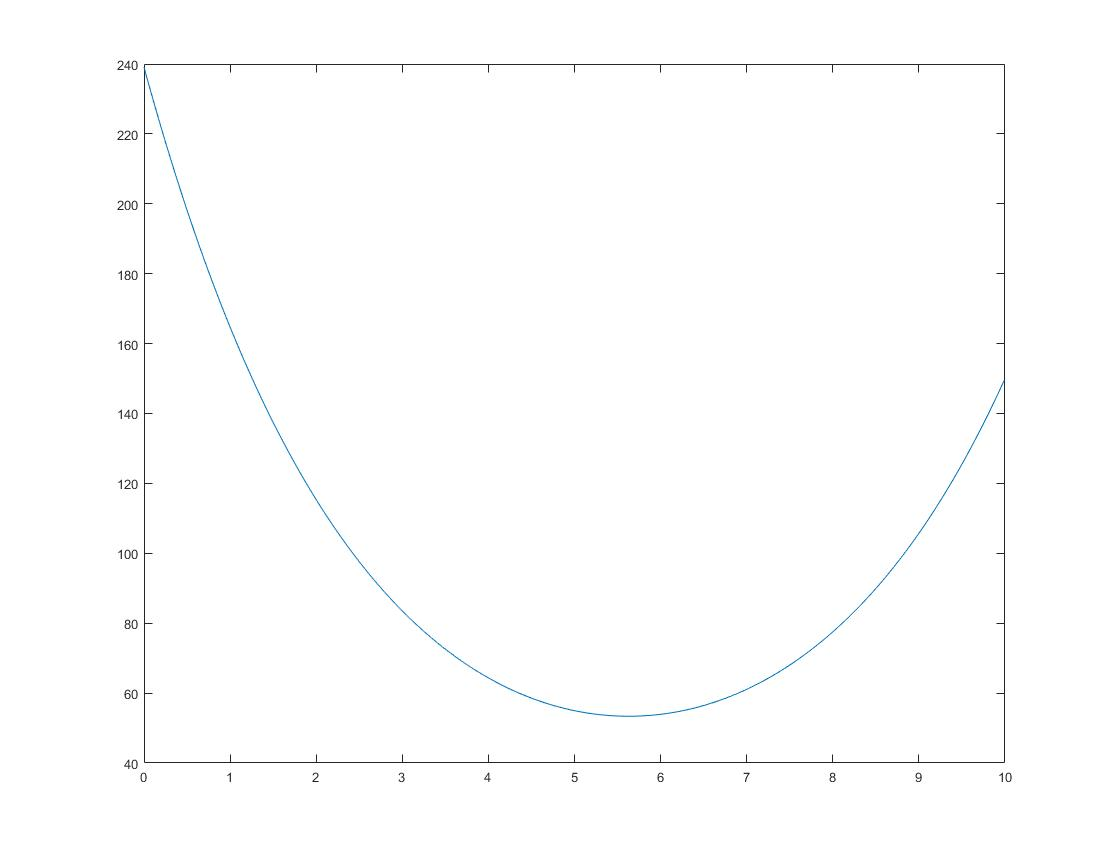
\includegraphics[width=\linewidth]{HW11-TriDiag.jpg}

\end{solution}

\setcounter{problem}{3}
\begin{problem}
Use the finite difference method to solve 
\[ 7\frac{d^{2}y}{dx^{2}} -2\frac{dy}{dx} -y +x =0 \]
with the boundary conditions $y(0)=5$ and $y(20)=8$, and $\Delta x=2$.
\end{problem}

\end{document}